\chapter{Implementation}
\section{Reaching a static target}
\subsection{The Problem} \label{static_target:the_problem}
A common task for an AI in a game is to reach a a given destination. According to \cite{alonso2020deeplearningnavigation} the common way to achieve this goal is by using \emph{navigation meshes} (NavMeshes). These are represented as graphs, and their nodes represent surfaces that can be traversed. Afterwards, algorithms such as \emph{A*} can be used to find the fastest way for an agent to go from point A to point B. However, these \emph{NavMeshes} require to be \emph{baked} in advance, so updating them in real time can prove to be a challenge depending on several factors such as:
% (TODO explicatie baked vezi \cite{alonso2020deeplearningnavigation})
\begin{itemize}
    \item the game engine used
    \item the complexity of the game environment
    \item the computational cost associated with recreating in real time these meshes
\end{itemize}

A proposed solution for this problem would be to use AI agents that have been trained using deep learning methods, in such a manner that they would be independent from changes to the environment.

\subsection{Implementing the solution} \label{static_target:implementation}
\paragraph{}
First, the action space for the agent is defined: due to the fact that we only need to move the agent to a given position, the action space consists of moving the agent forward or backward, and rotating it. Because the agent is supposed to be controlled by a controller, its movement input is defined as a real number in the $[-1, 1]$ interval for both $X$ and $Y$ axes. However, a discrete action space will be used instead of a continuous one to reduce the difficulty of learning, and also because there is no need for the agent to have movements that are so precise. For each axis the action space will be represented by the discrete space: $\{-1, -0.5, 0, 0.5, 1\}$.

\paragraph{}
To make decisions, the agent will need to make several observations about its surroundings. Firstly, it will need to know how close it is to certain objects in the environment. To accomplish this, several \emph{raycasts} will be used to measure the distance from the agent, similar to a \emph{LIDAR}. The raycasts start from the center of the agent and are spread in such a way that the angle between 2 consecutive rays is equal for any 2 consecutive rays. The observation will contain the distance until the rays hit an object. Also, the index of the layer of the hit object will be included in the observations, so that the agent will differentiate between regular environment objects and more important objects, such as other players, enemies, etc. For this implementation, 32 rays were used. A visual representation can be seen in Figure \ref{photo:tank_raycasts}

\begin{figure}
    \begin{center}
        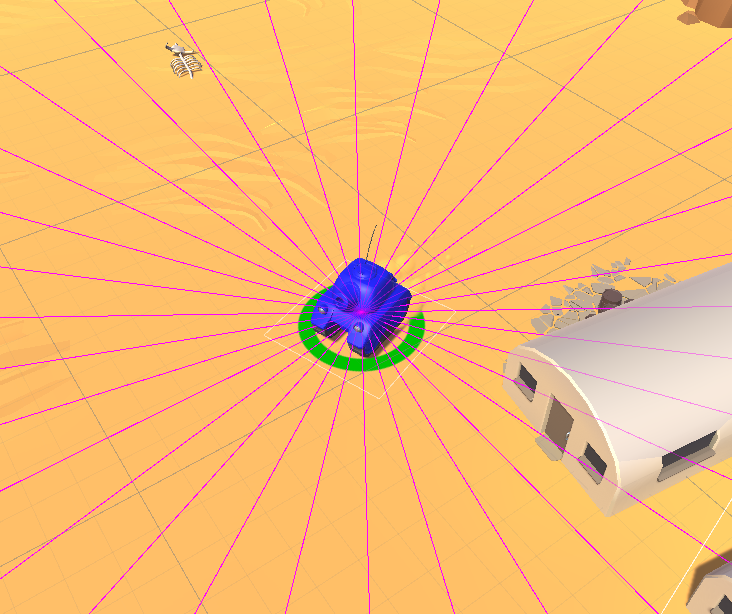
\includegraphics[width=0.7\linewidth]{tanks_2.png}
        \caption{The raycasts (in magenta) that are \emph{shot} by the agent}
        \label{photo:tank_raycasts}
    \end{center}
\end{figure}
% (TODO: add ceva despre lidar si un paper https://oceanservice.noaa.gov/facts/lidar.html)

Other observations that are made are the agent's position in space and also that of the target. This observation is included so that the agent can learn how movement brings it closer or further to the target. The next observation is the agent's forward vector so it can know in which direction it is moving. The optimal direction that the agent should take is also observed and obtained by computing the vector difference between the target's position and the agent's position. To know how much to adjust its trajectory, the angle between the agent's forward vector and the target is observed; the angle is signed so that the agent can learn to adjust its trajectory to the left or to the right. The distance to the target is added to the observations so that the agent can learn that when the distance is getting smaller it is rewarded. The agent's normalized velocity vector is observed to show in which direction it is moving based on the given input. The angle between the agent's velocity vector and its forward vector is observed to tell if the agent is moving forwards or backwards. Finally, the agent's velocity magnitude is observed so the agent can know if it is moving or standing still. 

In summary the following observations are being made:
\begin{itemize}
    \item distance for each raycast until it hits an object
    \item layer index of object hit by the raycast
    \item spatial postion of the agent
    \item spatial position of the target
    \item agent's forward vector
    \item optimal direction of the agent
    \item signed angle between the agent's forward vector and the target
    \item distance from the target
    \item agent's normalized velocity vector
    \item angle between the agent's velocity vector and its forward vector
    \item agent's velocity magnitude
\end{itemize}

\paragraph{}
In order for the agent to be able to learn to solve a specific problem, in this case, to reach a target, it must be rewarded or punished according to the actions that were taken. It is important to be mindful of the rewards that are given to the agent because only giving rewards and not punishing it can lead the agent to learn a behaviour that will maximize its reward, but will not be able to solve the problem, as it will be described shortly.

To begin, the first reward that was implemented, was the reward for reaching the objective, which is the goal of the agent and should also be a substantial reward. The other rewards that ware added were based on the direction of the movement and how close to the target it was, the reward increasing in value if the agent was closer to the objective (\ref{reward:1}) and a reward if the raycasts are hitting the destination object, which also increases in value if the agent is closer to the target (\ref{reward:2}). 

\begin{equation} \label{reward:1}
    R_\text{distance to target} = \frac{(1 - \frac{\alpha}{180}) \cdot r}{d}
\end{equation}
where:
\begin{itemize}
    % \item [$R_\text{dist to target}$]: is the obtained reward
    \item [$\alpha$]: is the angle between the agent's current direction and the optimal direction
    \item [$r$]: is the reward that is obtained if the agent has the optimal direction
    \item [$d$]: is the distance from the agent to the objective
\end{itemize}

\begin{equation} \label{reward:2}
    R_\text{ray distance} = \frac{r}{d_{i}}
\end{equation}
where:
\begin{itemize}
    % \item [$R_\text{ray dist}$]: is the obtained reward
    \item [$r$]: is the reward obtained if the distance between the agent and the objective is minimum
    \item [$d_{i}$]: is the obtained distance by the raycast $i$ from the agent to the object
\end{itemize}

However, these three rewards are not enough for the agent: through learning experiments it was observed that the agent was performing poorly: it would get stuck trying to move through a wall, it would never reach the objective and just spin around, or in some cases, it would just stand still.

To solve these problems, several punishments were implemented to correct the behavior of the agent. To prevent the agent for not moving, a constant penalty was added, to incentivise the agent to move towards the reward, so that it will receive a reward. Also, to comabat standing still, if the agent does not move, it receives an additional penalty, and if it does not move for more than 100 time steps, it receives a huge penalty and the episode ends. 

To stop the agent from trying to pass thorugh walls, a penalty is added if the raycasts that hit walls or other objects in the environment, have the distance to the hit object be a smaller than a given number. This penalty also increases the closer the agent gets to a wall (\ref{punishment:1}). 

\begin{equation} \label{punishment:1}
    R_\text{wall penalty} = \frac{p}{d_{i}}, \text{if } d_{i} < d
\end{equation}
where:
\begin{itemize}
    % \item [$R_\text{wall penalty}$]: is the obtained reward
    \item [$p$]: is the penalty obtained if the distance between the agent and the wall/environmental object is minimum
    \item [$d_{i}$]: is the obtained distance by the raycast $i$ from the agent to the object
    \item [$d$]: is the maximum distance for which the penalty is applied
\end{itemize}

Another penalty was added if the agent is moving away from objective, and as before, it increases the further away it gets from the objective (\ref{punishment:2}). 

\begin{equation} \label{punishment:2}
    R_\text{moving away} = \frac{\alpha}{180} \cdot p
\end{equation}
where:
\begin{itemize}
    % \item [$R_\text{moving away}$]: is the obtained reward
    \item [$p$]: is the penalty obtained if the distance between the agent and the wall/environmental object is minimum
    \item [$\alpha$]: is the angle between the agent's current direction and the optimal direction
\end{itemize}

Through training, two undesirable behaviours were observed: it was observed that the agent would sometimes make sudden jerky movments, trying to change its direction and immediatly returning to its previous trajectory, and that the agent would learn to drive backwards. To fix the first problem, a penalty was added if the agent would change its direction (\ref{punishment:3}), and to fix the second one, a penalty was added if the tank was moving backwards (\ref{punishment:4}).

\begin{equation} \label{punishment:3}
    R_\text{direction change} = \frac{\alpha}{180} \cdot p
\end{equation}
where:
\begin{itemize}
    % \item [$R_\text{dir change}$]: is the obtained reward
    \item [$p$]: is the penalty obtained for changing the movement direction
    \item [$\alpha$]: is the angle between the agent's current direction and its previous direction
\end{itemize}

\begin{equation} \label{punishment:4}
    R_\text{backwards} = \frac{\alpha}{180} \cdot p, \text{if } \alpha > 90
\end{equation}
where:
\begin{itemize}
    % \item [$R_\text{backwards}$]: is the obtained reward
    \item [$p$]: is the penalty obtained for moving backwards
    \item [$\alpha$]: is the angle between the agent's current direction and its forward vector
\end{itemize}

In summary, the used rewards and penalites and their values can be seen in Table \ref{reward_punish_table:1}.

\begin{table}
    \centering
    \begin{tabular}{|| m{15em} | m{4em} | m{15em} ||}
    \hline \hline
    \strong{Name} & \strong{Value} & \strong{Notes} \\ \hline \hline
    Reach Objective Reward & 10 &  \\ \hline
    Move Towards Objective Reward & 0.001 & is scaled by the distance between agent and objective \\ \hline
    Raycast Touches Objective Reward & 0.001 & is scaled by the distance between agent and objective \\ \hline
    Constant Penalty & -0.005 & is applied at each time step \\ \hline
    Not Moving Penalty & -0.05 &  \\ \hline
    Not Moving For 100 Steps Penalty & -50 &  \\ \hline
    Moving Towards Wall Penalty & -0.002 & is scaled by the distance between agent and object \\ \hline
    Moving Away From Objective Penalty & -0.025 & is scaled by the distance between agent and objective \\ \hline
    Sudden Movement Penalty & -0.01 & is scaled by the angle between the agent's current direction and its previous one \\ \hline
    Moving Backwards Penalty & -0.005 &  \\ \hline \hline
    \end{tabular}
    \caption{Rewards and Penalites}
    \label{reward_punish_table:1}
\end{table}

The final reward function can be expressed as:
\begin{equation}
    R = \mathbb{1}_\text{target} + \alpha + R_\text{distance to target} + R_\text{ray distance} + R_\text{wall penalty} + R_\text{moving away} + R_\text{direction change} + R_\text{backwards}
\end{equation}
where:
\begin{itemize}
    \item [$R$]: is the total reward
    \item [$\mathbb{1}_\text{target}$]: is the reward obtained for reaching the target
    \item [$\alpha$]: is the constant penalty
\end{itemize}


\subsection{Training} \label{static_target:training}

Each training session consisted of $10^7$ steps, and 30 agents were trained in parallel. The training times were between 3-4 hours. The agents are supposed to learn to reach an objective which appears in one of 17 predefined positions on the map. Once the agent reaches the objective, it is moved in another location chosen randomly. The objective is reprezented as a cuboid, as it can be seen in Figure \ref{photo:tank_chasing_target}, for better visualization of the training process. Each separate training instance uses the same seed for the random number generator, so that the objectives will appear in the same order for each of the training instances. Each training episode has a limit of $5000$ steps.

\begin{figure}
    \begin{center}
        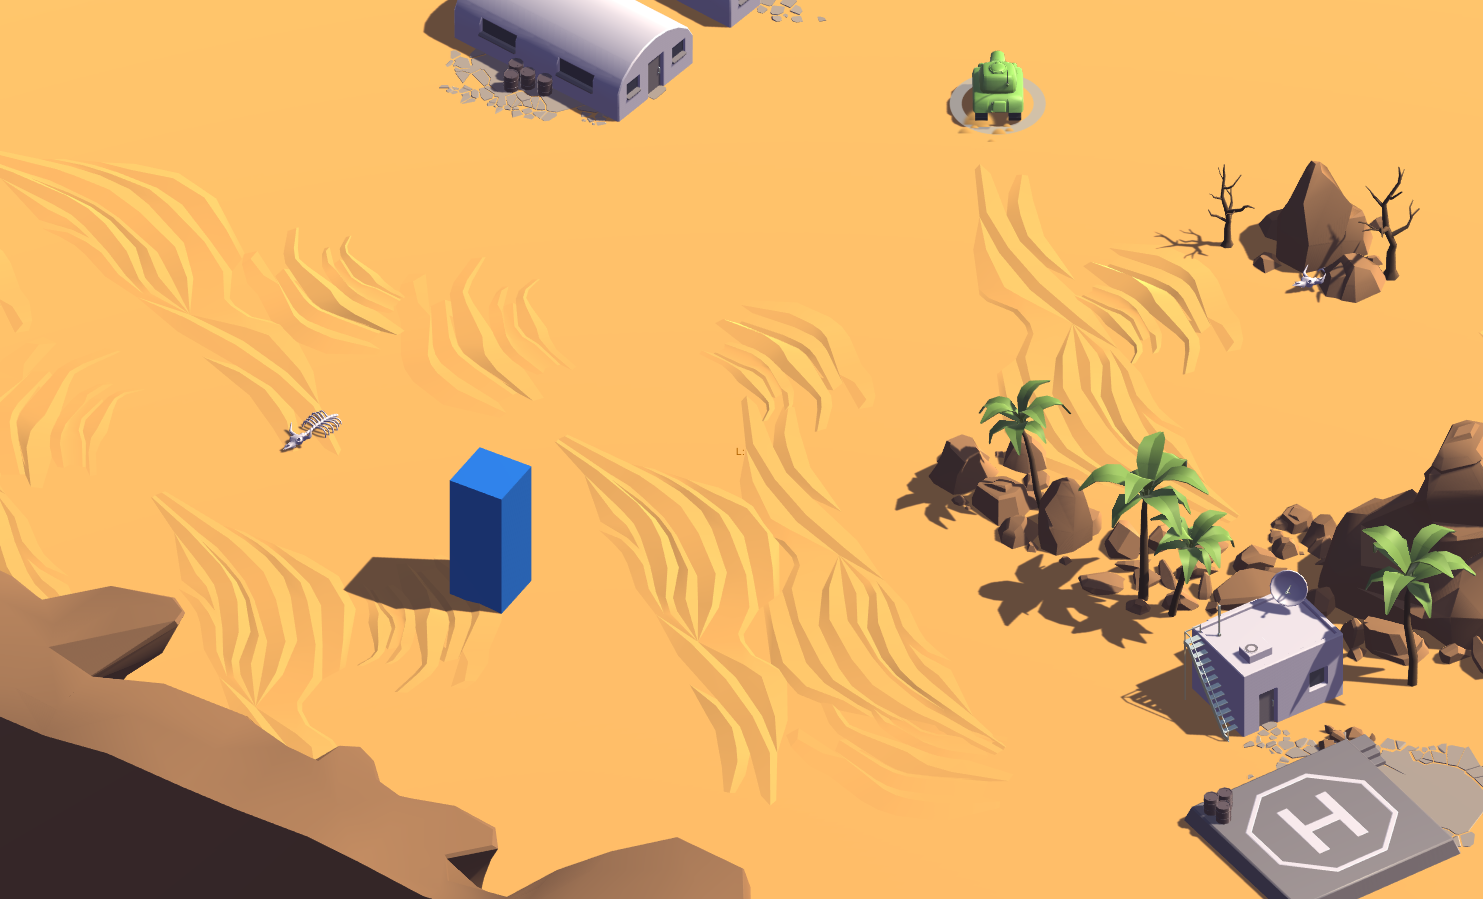
\includegraphics[width=0.8\linewidth]{tanks_3.png}
        \caption{Photo of agent (green) and the target that it is supposed to reach (blue)}
        \label{photo:tank_chasing_target}
    \end{center}
\end{figure}

In the initial training sessions, the agents were unable to learn to reach the objective, becoming stuck rotating in a circle. A proposed solution was to keep the objective in the same position until the agent reaches it 30 times. After reaching the objective 30 times, the objective would start appearing in the random predefined locations. This was done to possibly kickstart the agent's learning process, but the approach failed, the agent being unable to learn to reach the objective. Another approach was to increase the neural network's size, however this approach prove unsuccessful as well. The approach that worked was to remove the agent's postion and the objective's position from the observations. 
% TODO: sa zic de curiosity

The agent's training process was done using multiple neural network configurations, including different number of network layers ($1$, $3$, $5$, $7$) and different number of units per layer ($128$, $256$, $512$).

The hyperparameters used for the training can be seen in Table \ref{static_target_hyperparameters}.
\begin{table}
    \centering
    \begin{tabular}{|| m{10em} | m{10em} ||}
        \hline \hline
        \strong{Hyperparameter} & \strong{Value} \\ \hline \hline
        Gamma & 0.9 \\ \hline
        Lambda & 0.95 \\ \hline
        Beta & 0.005 \\ \hline
        Epsilon & 0.2 \\ \hline
        Buffer Size & 8192 \\ \hline
        Batch Size & 256 \\ \hline
        Number of Epochs & 3 \\ \hline
        Learning Rate & 0.0003 \\ \hline \hline
    \end{tabular}
    \caption{Training hyperparameters}
    \label{static_target_hyperparameters}
\end{table}

\paragraph{}
The results for training the agent with 1 network layer can be seen in Figure \ref{train_results_static_1_layers}, and in Table \ref{move_to_static_targets_table:1}. In this case, the configuration with $256$ units was not able to be trained properly, remaining stuck moving in a circle. Between the two configurations that were successfully trained, it can be seen that the one with $128$ units, performed better during the training process than the one with $512$ units, obtaining, at the end, a mean reward that is higher by $18.79\%$.


\begin{figure}
    \begin{center}
        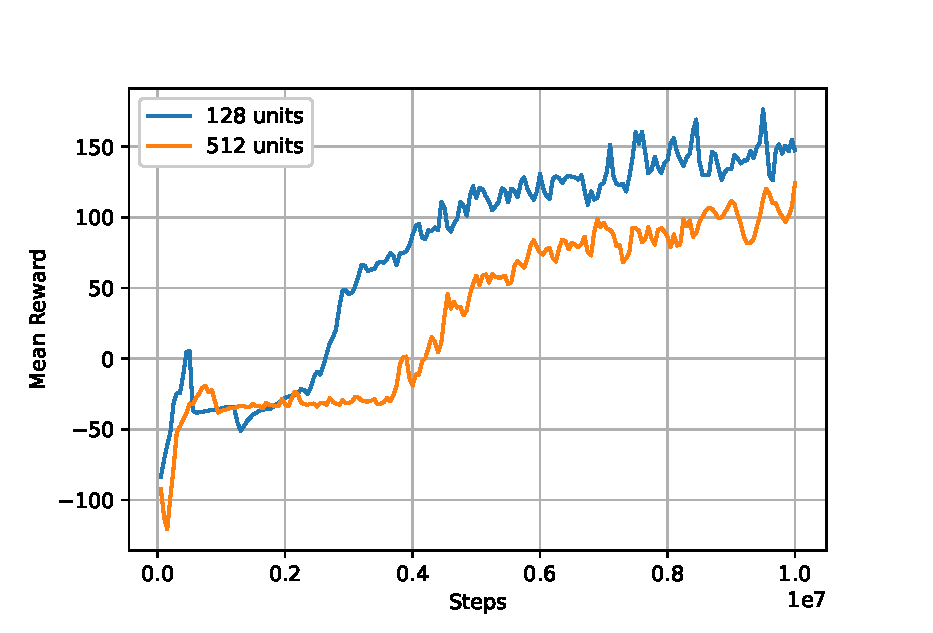
\includegraphics[width=0.95\linewidth]{move_to_static_target_1_layers.eps}
        \caption{Training results for reaching a static target with a network with 1 hidden layer}
        \label{train_results_static_1_layers}
    \end{center}
\end{figure}


% \paragraph{}
The results for training the agent with 3 network layers can be seen in Figure \ref{train_results_static_3_layers}, and in Table \ref{move_to_static_targets_table:1}. From these results, it can be seen that the configurations with $128$ and $256$ units, performed very similarily during the training, however, the one with $512$ units started to lag behind these two at around $4 \cdot 10^6$ steps. Again, the configuration with the least units had the best training results, obtaining a result that is $2.61\%$ better than the one with with $256$ units and better by $29\%$ than the one with $512$ units. 

\begin{figure}
    \begin{center}
        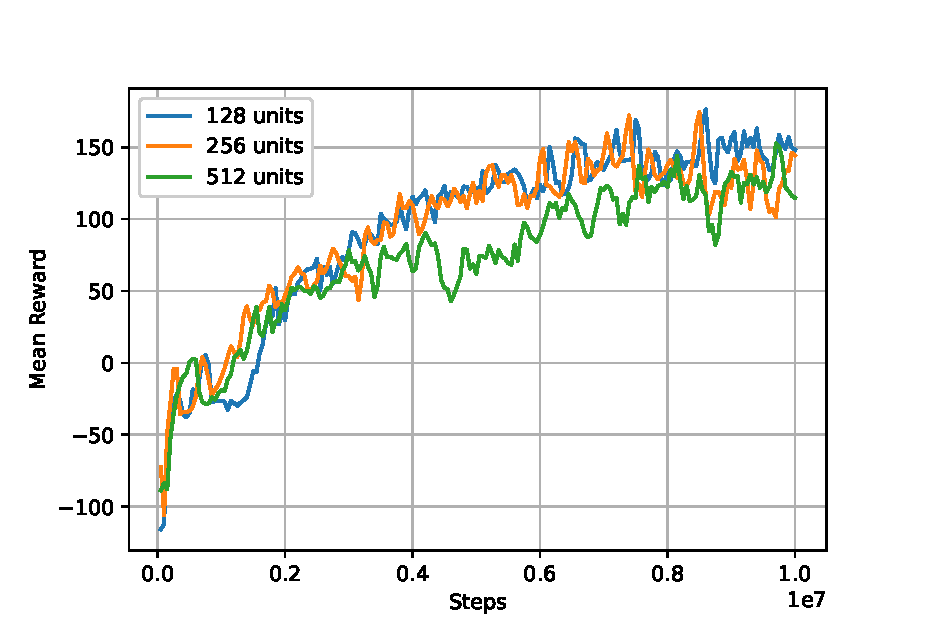
\includegraphics[width=0.95\linewidth]{move_to_static_target_3_layers.eps}
        \caption{Training results for reaching a static target with a network with 3 hidden layers}
        \label{train_results_static_3_layers}
    \end{center}
\end{figure}


% \paragraph{}
Results for training the agent with 5 network layers can be seen in Figure \ref{train_results_static_5_layers}, and in Table \ref{move_to_static_targets_table:1}. From the training results, it can be seen that in the later stages, the configuration with $256$ units falls behind the other two. Unlike the results with 1 layer and 3 layers, the best performing configuration is the one with $512$ units per layer, being better by $8.72\%$ than the configuration with $128$ units, and by $35.45\%$ than the configuration with $256$ units.

\begin{figure}
    \begin{center}
        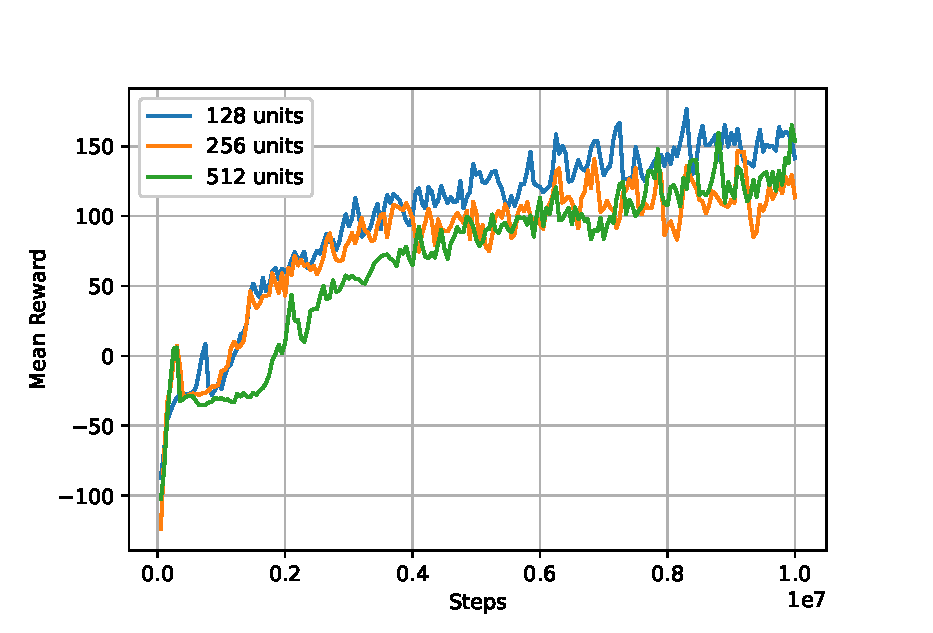
\includegraphics[width=0.95\linewidth]{move_to_static_target_5_layers.eps}
        \caption{Training results for reaching a static target with a network with 5 hidden layers}
        \label{train_results_static_5_layers}
    \end{center}
\end{figure}

% \paragraph{}
Results for training the agent with 7 network layers can be seen in Figure \ref{train_results_static_7_layers}, and in Table \ref{move_to_static_targets_table:1}. From the training results it can be seen that the configuration with $128$ units per layer performs better than the other two, but at the final stages of the training, it is caught up to by the configuration with $256$ units. In the end, the configurations with $128$ and $256$ units per layer had virtually identical results at the end of the training, and were better by $\sim36.3\%$ than the one with $512$ units.

\begin{figure}
    \begin{center}
        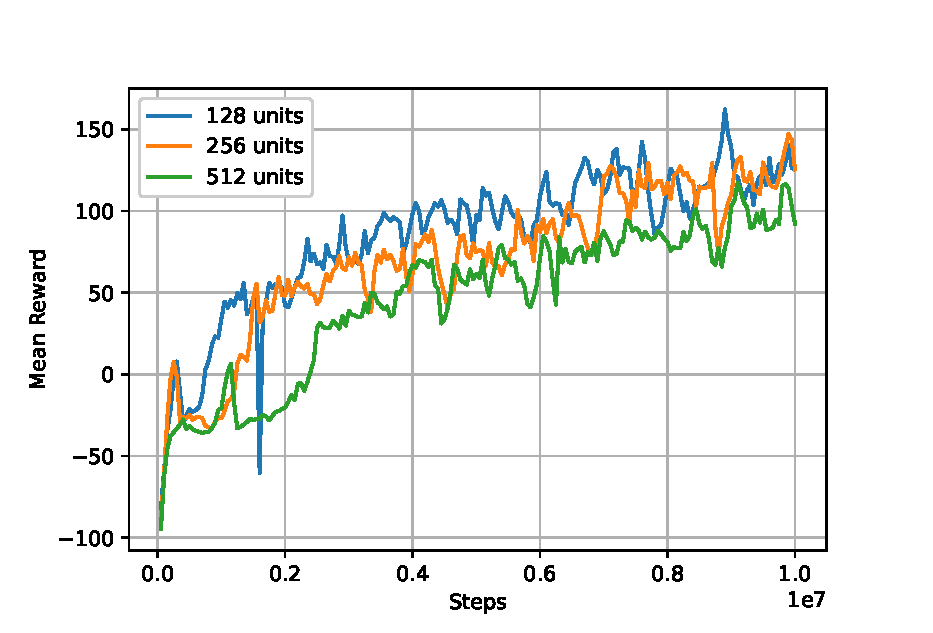
\includegraphics[width=0.95\linewidth]{move_to_static_target_7_layers.eps}
        \caption{Training results for reaching a static target with a network with 7 hidden layers}
        \label{train_results_static_7_layers}
    \end{center}
\end{figure}

\paragraph{}
All the training results can be seen in Table \ref{move_to_static_targets_table:1} and in Figure \ref{train_results_static_bar_chart}. It can be observed that network configurations with a smaller number of units per layer obtained better training results than the others. This could be due to the fact that the problem is not a very complex one, and because a smaller network can be trained faster. The configurations with 1, 3, or 5 layers obtained similar results, however, when 7 layers are used, there is a noticeable decrease in the agent's performance. These being said, from the training results it seems that using a network configuration with less layers and less units per layer offers almost the best result, thus it is the most practical one to be used, since it uses the least computing resources. Using larger networks should be done by training the agent for longer periods of time. However, it is possible when using a smaller network to obtain an unusable model, as was the case in this experiment using a network configuration with 1 hidden layer and 256 units per layer.

\begin{table}
    \centering
    \begin{tabular}{|| m{15em} | m{15em} ||}
    \hline \hline
    \strong{Network Configuration} & \strong{Final Mean Reward} \\ \hline \hline
    1 layer, 128 units & 147.568 \\ \hline
    1 layer, 256 units & DNF \\ \hline
    1 layer, 512 units & 124.221 \\ \hline
    3 layers, 128 units & 148.136 \\ \hline
    3 layers, 256 units & 144.366 \\ \hline
    3 layers, 512 units & 114.828 \\ \hline
    5 layers, 128 units & 141.369 \\ \hline
    5 layers, 256 units & 113.478 \\ \hline
    5 layers, 512 units & 153.709 \\ \hline
    7 layers, 128 units & 125.727 \\ \hline
    7 layers, 256 units & 125.441 \\ \hline
    7 layers, 512 units & 92.128 \\ \hline \hline
    \end{tabular}
    \caption{Final training results for reaching a static target}
    \label{move_to_static_targets_table:1}
\end{table}

\begin{figure}
    \begin{center}
        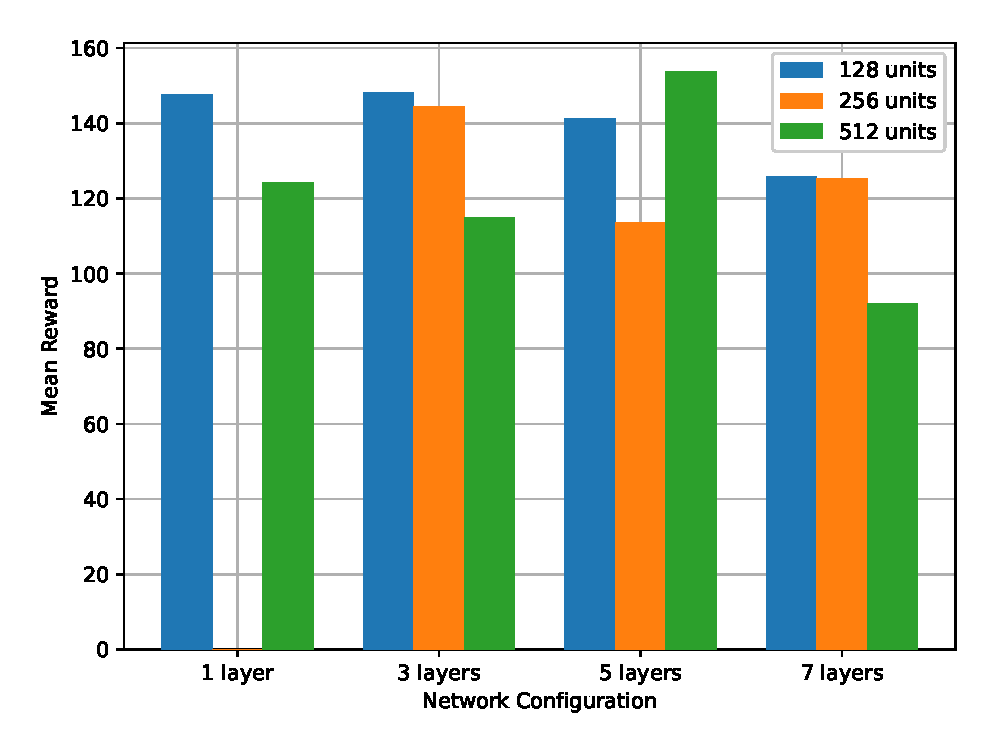
\includegraphics[width=\linewidth]{move_to_static_target_bar_chart.eps}
        \caption{Training results for all network configurations for reaching a static target}
        \label{train_results_static_bar_chart}
    \end{center}
\end{figure}



% =====================================



\section{Reaching a moving target}


\subsection{The Problem} \label{moving_target:the_problem}
Another standard behavior of an AI in video games is to be able to chase a target, so that it can, maybe, perform a specific action once the object controlled by the AI is close enough to the target . A simple way to achieve this behavior would be to use a \emph{NavMesh} and periodically change the agent's destination. Compared to the problem described at \ref{static_target:the_problem}, the addition here is that the agent has to recompute its route at specified intervals.
% (TODO: sa mai dezvolt asta)

\paragraph{}
Again, the proposed solution would be to use AI agents that are trained using deep learning methods.

\subsection{Implementing the solution} \label{moving_target:implementation}
The basic implementation for this problem is the same as the one described at \ref{static_target:implementation}, with the same observations, rewards and penalties being used. The addition would be to add an observation that is the direction in which the target is moving. This can be used by the agent to predict in which direction the target is moving and to eventually intercept it along its trajectory. Another idea would be to add memory to the agent, in the form of LSTM, so that it can achieve this result in a more \emph{natural} way.

\subsection{Training} \label{moving_target:training}
The training is similar to the process described at \ref{static_target:training}, with the same number of agents being trained at the same time, same number of steps, same hyperparameters (Table \ref{static_target_hyperparameters}), etc. 

Trying to add memory to the agent was a failure, the agent being unable to learn to chase the target, and getting stuck moving in a circle. This behaviour happened even when changing the recurrent network's hyperparameters \emph{sequence length} and \emph{memory size}. 
% (TODO: maybe add some combinations)

Training this agent was done in 2 separate ways: one where the target's direction is not in the observations, and one where it is. The first round of training is done without the observation that was mentioned previously.

\paragraph{}
Results for training the agent with a single network layer and without the target's direction obsrevation can be seen in Figure \ref{train_results_moving_1_layers} and Table \ref{move_to_moving_targets_table:1}. From these results it can be seen that all 3 configurations performed virtually identically, and at the end of the training had obtained the same mean reward.

\begin{figure}
    \begin{center}
        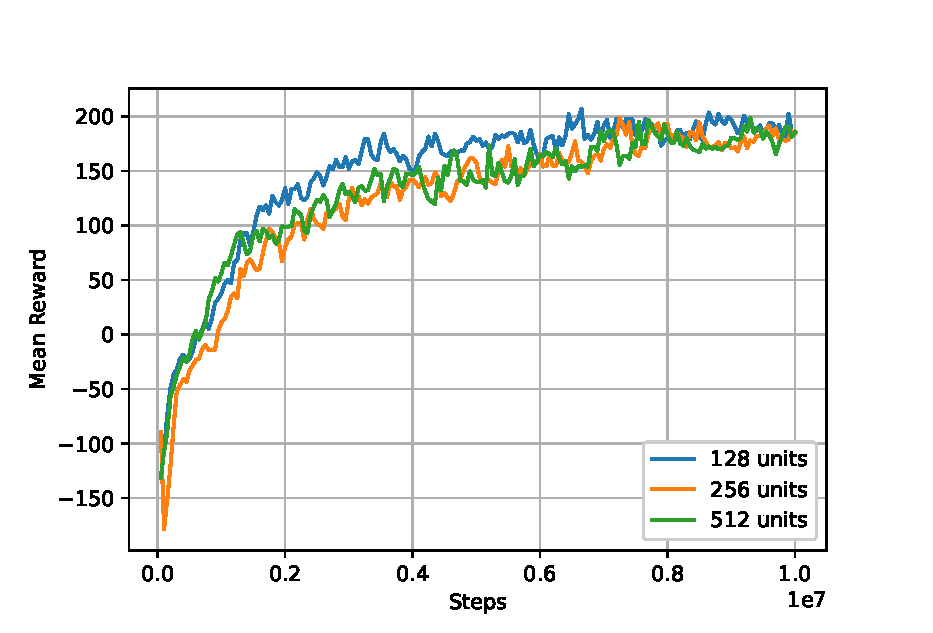
\includegraphics[width=0.95\linewidth]{move_to_moving_target_1_layers.eps}
        \caption{Training results for reaching a moving target with a network with 1 hidden layer}
        \label{train_results_moving_1_layers}
    \end{center}
\end{figure}


Results for training the agent with 3 network layers and without the target's direction obsrevation can be seen in Figure \ref{train_results_moving_3_layers} and Table \ref{move_to_moving_targets_table:1}. In these results, it seems that the configuration with $128$ units obtains better results during training than the configuration with $256$ units, which in turn obtains better results than the one with $512$ units. At the end of the training, the configuration with $128$ units is better by $1.02\%$ than the one with $256$ units and better by $28.58\%$ than the one with $512$ units.

\begin{figure}
    \begin{center}
        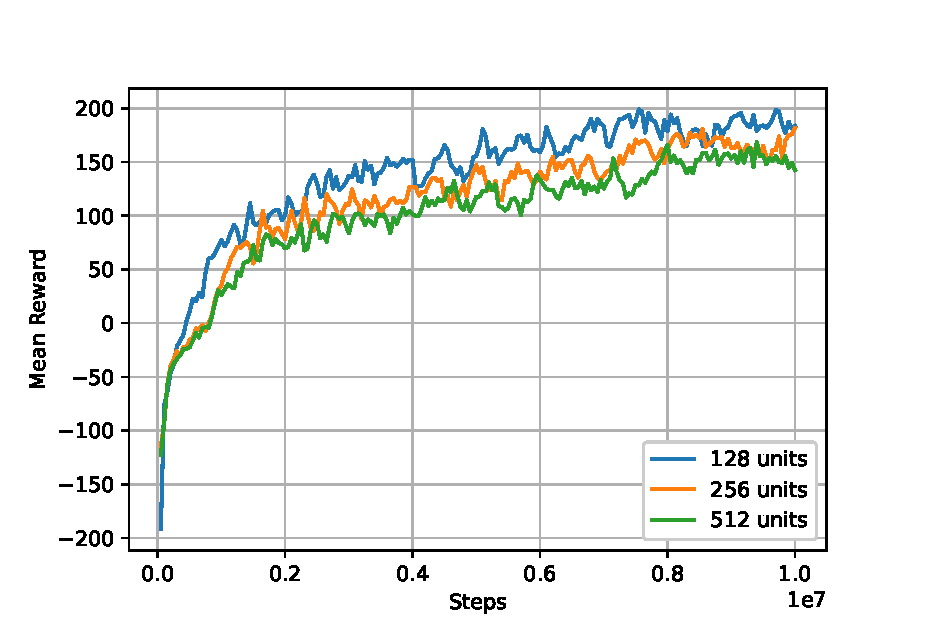
\includegraphics[width=0.95\linewidth]{move_to_moving_target_3_layers.eps}
        \caption{Training results for reaching a moving target with a network with 3 hidden layers}
        \label{train_results_moving_3_layers}
    \end{center}
\end{figure}


Results for training the agent with 5 network layers and without the target's direction obsrevation can be seen in Figure \ref{train_results_moving_5_layers} and Table \ref{move_to_moving_targets_table:1}. The results during training are similar to the configuration with 3 layers, with the configuration with $128$ units being better than the other two. The final result is that the configuration with $128$ units is better by $8.87\%$ than the one with $256$ units and better by $17.9\%$ than the one with $512$ units.

\begin{figure}
    \begin{center}
        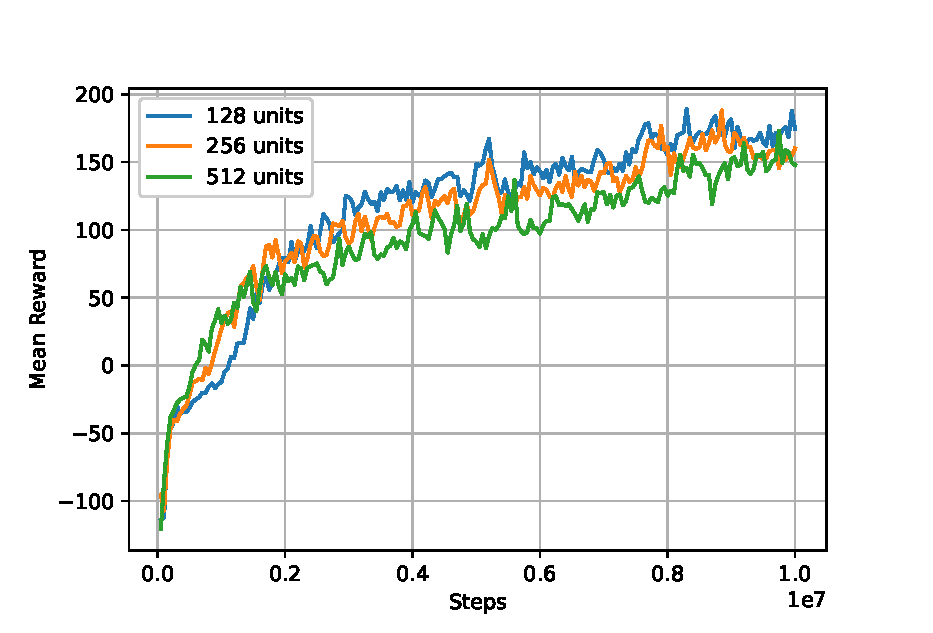
\includegraphics[width=0.95\linewidth]{move_to_moving_target_5_layers.eps}
        \caption{Training results for reaching a moving target with a network with 5 hidden layers}
        \label{train_results_moving_5_layers}
    \end{center}
\end{figure}


\paragraph{}
The second round of training is done by adding the target's movement direction to the agent's observations.

The results for training the agent with a single network layer and without the target's direction obsrevation can be seen in Figure \ref{train_results_moving_1_layers_with_dir} and Table \ref{move_to_moving_targets_table:1}. As in the previous cases, the best performed configuration during training is the one with the least units, i.e. 128 units. This one is better by $39.47\%$ than the configuration with 256 units, and by $6.88\%$ than the one with 512 units.

\begin{figure}
    \begin{center}
        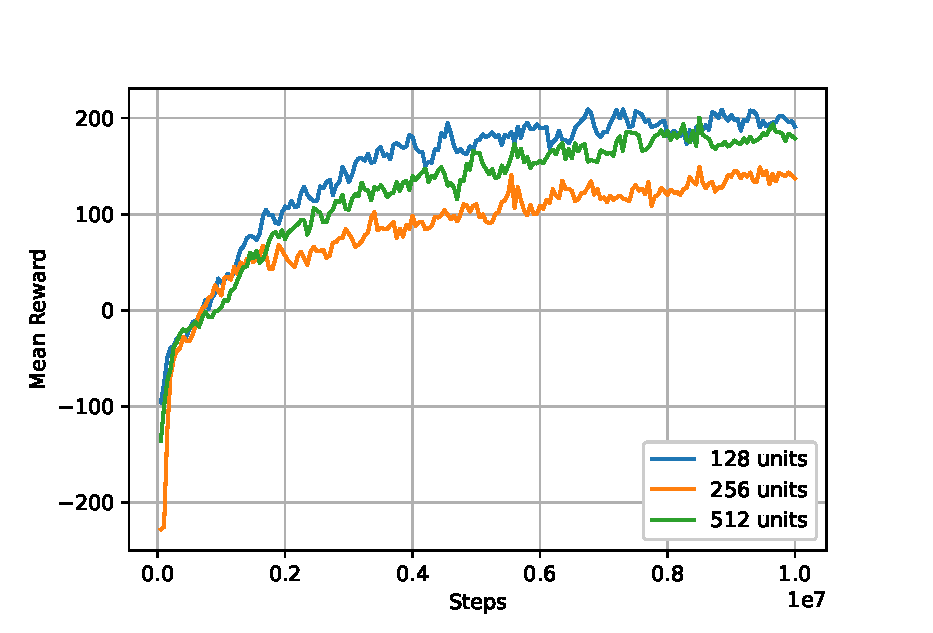
\includegraphics[width=0.95\linewidth]{move_to_moving_target_1_layers_with_dir.eps}
        \caption{Training results for reaching a moving target with a network with 1 hidden layer and with observation of target's direction}
        \label{train_results_moving_1_layers_with_dir}
    \end{center}
\end{figure}

Training the agent with a network with 3 layers obtains the results that can be seen in Figure \ref{train_results_moving_3_layers_with_dir} and Table \ref{move_to_moving_targets_table:1}. This time, all 3 configuration performed very similarily during training. The best configuration here was the one with 512 units which was better by $4.99\%$ than the one with 128 units, and by $7.37\%$ than the one with 256 units.

\begin{figure}
    \begin{center}
        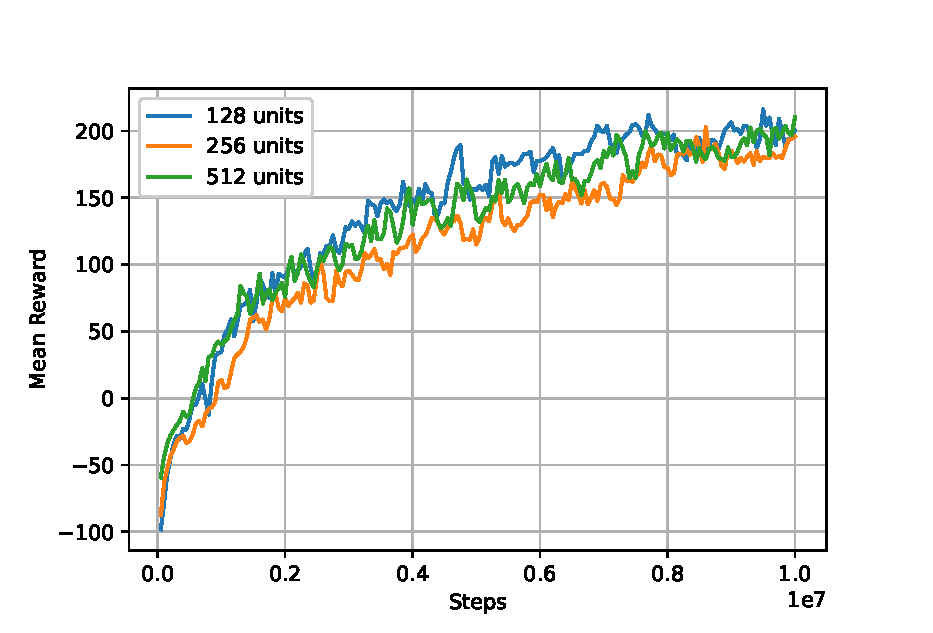
\includegraphics[width=0.95\linewidth]{move_to_moving_target_3_layers_with_dir.eps}
        \caption{Training results for reaching a moving target with a network with 3 hidden layers and with observation of target's direction}
        \label{train_results_moving_3_layers_with_dir}
    \end{center}
\end{figure}

Results for training the agent with 5 network layers and without the target's direction obsrevation can be seen in Figure \ref{train_results_moving_5_layers_with_dir} and Table \ref{move_to_moving_targets_table:1}. It can be observed that the configuration with 128 units outperforms the other two during training, the ohter two performing mostly identically until the final training steps, where the one with 512 units slightly overtakes the one with 128 units. The configuration with 512 units is better by $1.26\%$ than the one with 128 units and better by $17.93\%$ than the one with 256 units.

\begin{figure}
    \begin{center}
        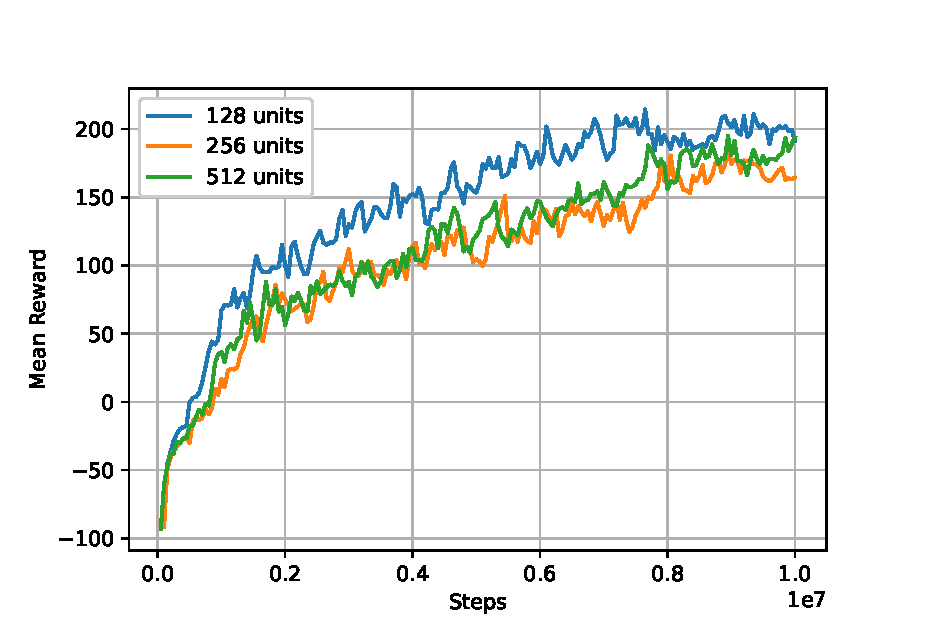
\includegraphics[width=0.95\linewidth]{move_to_moving_target_5_layers_with_dir.eps}
        \caption{Training results for reaching a moving target with a network with 5 hidden layers and with observation of target's direction}
        \label{train_results_moving_5_layers_with_dir}
    \end{center}
\end{figure}


\paragraph{}
Looking at the final results in Figure \ref{train_results_moving_bar_chart} and Table \ref{move_to_moving_targets_table:1} we can observe that the best netowrk configurations have either 128 units per layer or 512 units per layer. When increasing the number of layers and not using the target's movement direction as an observation, the agent's performance slightly decreased during the training. Adding the target's movement direction as an observation increases the performance of the agent, compared to the configuration with the same number of layers and without this observation. 

In conclusion, from these training results, it seems that adding the target's moving direction to the observations improves the agent's performance, the best results are achieved with either 128 or 512 units per hidden layer, and the best number of hidden layers is 3. The difference between using 128 units instead of 512 is a $\sim5\%$ decline in the agent's performance. If there are no reasons to reduce resource usage, the configuration with 3 hidden layers and 512 units per layer should be used.

\begin{table}
    \centering
    \begin{tabular}{|| m{11.3em} | m{10em} | m{9.6em} ||}
    \hline \hline
    \strong{Network Configuration} & \strong{Observed target's direction} & \strong{Final Mean Reward} \\ \hline \hline
    1 layer, 128 units & No & 184.547 \\ \hline
    1 layer, 128 units & Yes & 191.184 \\ \hline
    1 layer, 256 units & No & 184.563 \\ \hline
    1 layer, 256 units & Yes & 137.075 \\ \hline
    1 layer, 512 units & No & 185.936 \\ \hline
    1 layer, 512 units & Yes & 178.876 \\ \hline
    3 layers, 128 units & No & 183.288 \\ \hline
    3 layers, 128 units & Yes & 200.502 \\ \hline
    3 layers, 256 units & No & 181.435 \\ \hline
    3 layers, 256 units & Yes & 196.064 \\ \hline
    3 layers, 512 units & No & 142.54 \\ \hline
    3 layers, 512 units & Yes & 210.524 \\ \hline
    5 layers, 128 units & No & 174.404 \\ \hline
    5 layers, 128 units & Yes & 191.399 \\ \hline
    5 layers, 256 units & No & 159.966 \\ \hline
    5 layers, 256 units & Yes & 164.351 \\ \hline
    5 layers, 512 units & No & 147.922 \\ \hline
    5 layers, 512 units & Yes & 193.828 \\ \hline \hline
    \end{tabular}
    \caption{Final training results for reaching a moving target}
    \label{move_to_moving_targets_table:1}
\end{table}

\begin{figure}
    \begin{center}
        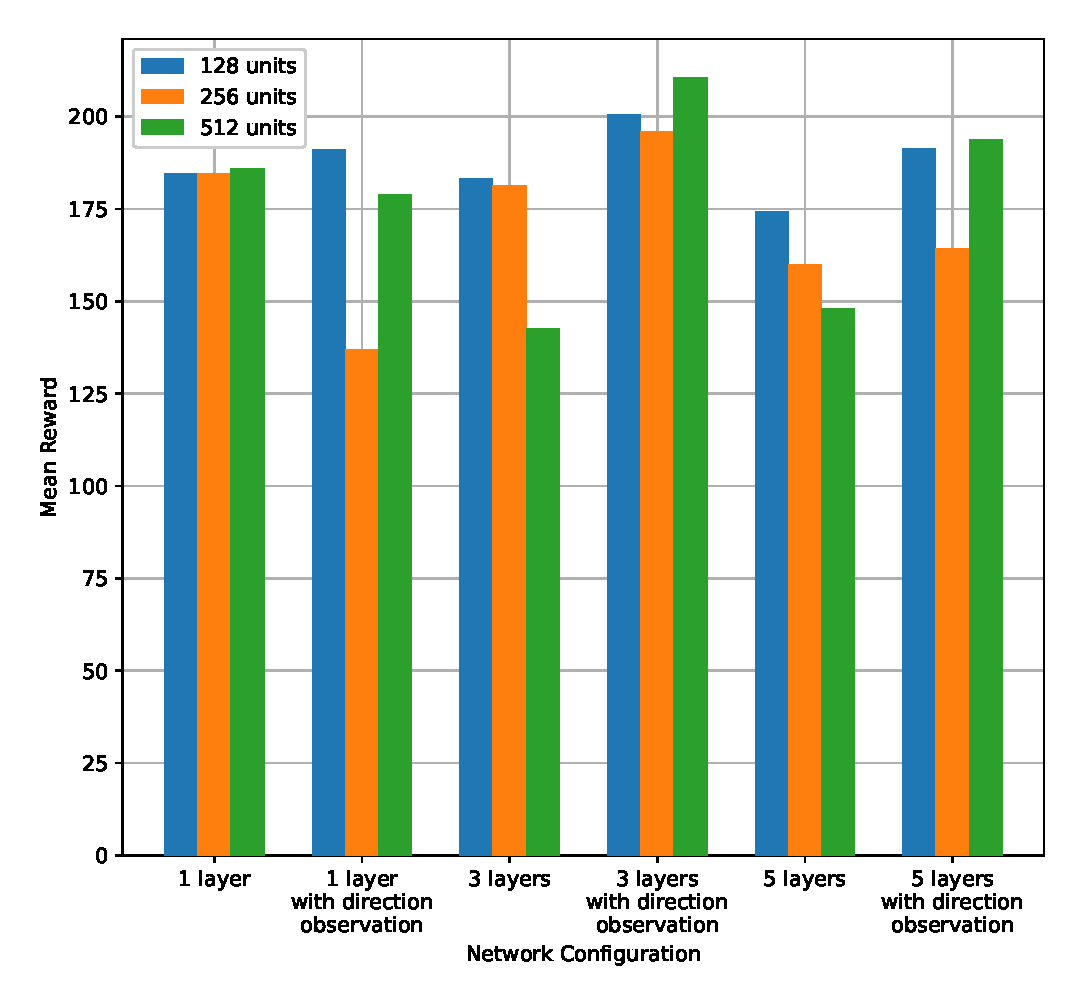
\includegraphics[width=\linewidth]{move_to_moving_target_bar_chart.eps}
        \caption{Training results for all network configurations for reaching a moving target}
        \label{train_results_moving_bar_chart}
    \end{center}
\end{figure}



% ===============================================



\section{Shooting a moving target}

\subsection{The Problem}

Another common use of AIs in gaming is to provide an opponent for the player, in this case to fight against. This brings a whole new dimension to the problem besides having the AI move in the given worldspace. Now, the AI must find the target, then be able to shoot at it, and also try to defend itself against the target, here by not getting hit by it. The AI must also be \emph{defeatable}, since providing players with an opponent that can always take the best course of action and being superior in every way to the human player does not constitute a fun experience. By not being \emph{perfect}, the human has a chance to defeat the AI, thus having a pleasant gaming experience. Balancing an AI to provide a good experience for a human player is out of the scope of this paper, the goal here being to manage to train an agent that can fight and eventualy win against an opponent. However, the agent should act in a way so that it could be actually used in a game. This would consist of acting more \emph{humanlike}, and less like a predictable computer program.
% (TODO: more research pe cacatu asta)

\subsection{Implementing the solution}

The implementation builds on what was described in Sections \ref{static_target:implementation} and \ref{moving_target:implementation}. The addition is that the agent does not need to reach a certain target, but to shoot it. For this, several aspects need to be changed to implement the bullet logic.

\paragraph{}
For starters, the agent's action space was increased from 2 branches to 4 branches. The first 2 branches will still handle the agent's movement, the third branch can have two values: 0 or 1, and this tells the agent if he should fire a bullet, and the fourth branch sets the bullet's shooting force, which can have 3 values: low, medium, or high.

\paragraph{}
Another change that was made, was adding new observations, most of them being related to the bullet. The first one is a flag that tells if the bullet is fired. The second one is the bullet's trajectory, which can be used by the agent to learn to shoot on target. The third observation is about the bullet's speed so that the agent can learn with what force the bullet has been shot. The final new observation, which is not related to the bullet, is the angle between the target's front vector and the vector from the target to the agent. This is used so that the agent can learn when it is in the target's crosshairs, and to possibly learn how to flank the target. 

In summary, the following observations have been added:
\begin{itemize}
    \item bullet is fired or not
    \item bullet's trajectory vector
    \item bullet's speed
    \item angle between the target's front vector and vector from target to the agent
\end{itemize}


\paragraph{}
Finally, new rewards and punishments were implemented. Firstly, the agent is no longer rewarded if it touches the target, it has to hit it with a bullet. To incentivise firing a bullet, a small reward is received when firing a bullet. Also, a penalty is added if the bullet misses the target, and disappears because it has travelled a certain distance, or it hit an environmental object. The other bullet reward that was added is a reward that is based on the bullet's trajectory and how close it is to the optimal trajectory to the target and is scaled by the distance from the bullet to the target, with the reward increasing the closer the bullet gets to the target. This reward is defined using Formula \ref{bullet:1}:

\begin{equation} \label{bullet:1}
    R_\text{bullet trajectory} = \frac{(1 - \frac{\alpha}{180}) \cdot r}{d} \cdot 2
\end{equation}
where:
\begin{itemize}
    % \item [$R_\text{bullet trajectory}$]: is the obtained reward
    \item [$\alpha$]: is the angle between the bullet's current trajectory and the optimal trajectory
    \item [$r$]: is the reward that is obtained if the bullet has the optimal trajectory
    \item [$d$]: is the distance from the bullet to the target
\end{itemize}

Two punishments were added to help the agent learn as if it were fighting a real opponent. The first one makes the agent stay at a given distance from the target, so that the agent will not try to stay glued to the target while trying to shoot it. This punishment is computed using Fomrula \ref{punishment:shoot_1}:

\begin{equation} \label{punishment:shoot_1}
    R_\text{desired distance} = \begin{cases}
        \frac{d - d'}{50} \cdot p & \text{for } d \geq d' \\
        \frac{p}{d} & \text{else}
    \end{cases}
\end{equation}
where:
\begin{itemize}
    % \item [$R$]: is the obtained reward
    \item [$d$]: is the distance from the agent to the target, that is clamped in the interval $[0, 50]$
    \item [$d'$]: is the desired distance from the agent to the target
    \item [$p$]: is the penalty for the agent not being at desired distance $d'$ from the target
\end{itemize}

The second punishment is applied when the agent is in front of the target, which means that the target can attack it. This punishment is added to try and teach the agent that it should flank its target so that it can attack it while being safe from being shot at. The punishment is computed using Formula \ref{punishment:shoot_2}

\begin{equation} \label{punishment:shoot_2}
    R_\text{in target's crosshair} = (1 - \frac{\alpha}{180}) \cdot p
\end{equation}
where:
\begin{itemize}
    % \item [$R$]: is the obtained reward
    \item [$\alpha$]: is the angle between the target's forward vector and the vector from the target to the agent
    \item [$p$]: is the penalty for being in front of the target
\end{itemize}

In addition to the rewards and penalties already being used, described in Table \ref{reward_punish_table:1}, the new ones have the following values:

\begin{table}
    \centering
    \begin{tabular}{|| m{15em} | m{4em} | m{15em} ||}
    \hline \hline
    \strong{Name} & \strong{Value} & \strong{Notes} \\ \hline \hline
    Shoot Target Reward & 10 &  \\ \hline
    Fire Bullet Reward & 0.1 & \\ \hline
    Bullet's Trajectory is Optimal Reward & 0.001 & is scaled by the distance between bullet and target \\ \hline
    Miss Target Penalty & -0.1 &  \\ \hline
    Agent Not At Desired Distance Penalty & -0.005 & is scaled by the difference of the desired distance and distance between agent and object \\ \hline
    Agent In Front Of Target Penalty & -0.05 & is scaled by the angle between the target's front vector and the vector from the target to the agent \\ \hline \hline
    \end{tabular}
    \caption{New Rewards and Penalites for agent that is shooting a moving target}
    \label{reward_punish_table:2}
\end{table}


\subsection{Training}

The agent's training was done in 2 ways: a naive way, where the agent is only rewarded if it manages to shoot the target, without regards with its positioning, and a more \emph{tactical} way where the agent is punished for not keeping distance between it and the target, and also for being in front of the target. These two approaches are documented at \ref{subsubsection:shoot_naive} and \ref{subsubsection:shoot_tactical} respectively.

\subsubsection{Naive approach} \label{subsubsection:shoot_naive}

As mentioned above, this approach only cares about the agent shooting the target, and not necessarily about the agent's positioning in relation to the target. This means that the penalties described in Formulae \ref{punishment:shoot_1} and \ref{punishment:shoot_2} are not applied. However, the reward concerning the bullet's trajectory described in Formula \ref{bullet:1} is used. The observations regarding the bullet (if the bullet is fired, the bullet's trajectory vector and its speed) are used, while the observation regarding the angle between the target's front vector and vector from target to the agent is unused.

It is also worth noting that during the first trainings, the only observation regarding the bullet that was used is the one that tells if the bullet is fired.

\paragraph{}
Results for training the agent with a single network layer can be seen in Figure \ref{train_results_shoot_1_layers} and Table \ref{shoot_moving_targets_table:1}. As with the previous agents, the best performing configuration during training is the one with 128 units per layer, while the other two lag behind it. The configuration with 128 units was better by $32.12\%$ than the one with 256 units, and better by $10\%$ than the one with 512 units.

\begin{figure}
    \begin{center}
        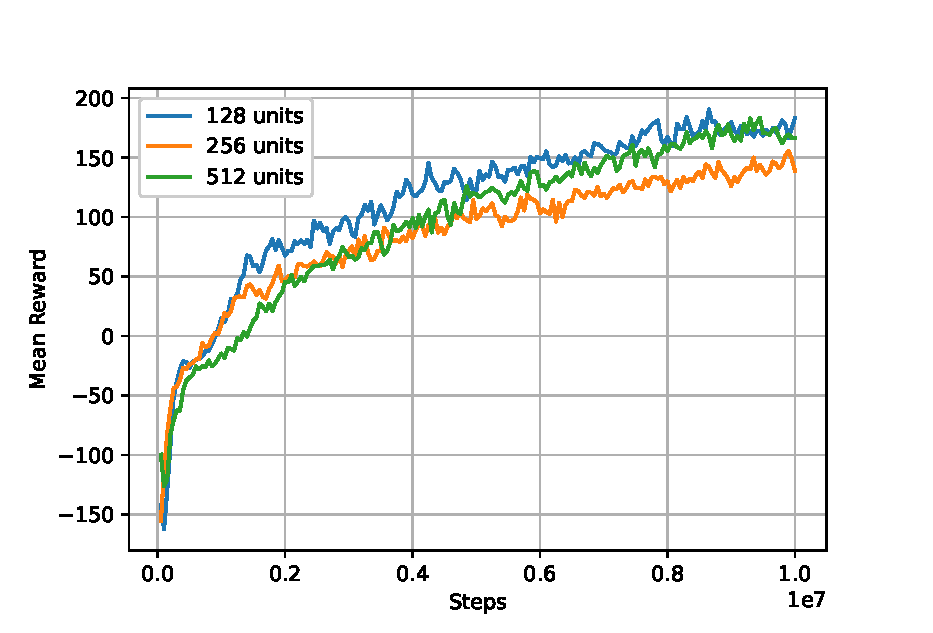
\includegraphics[width=0.95\linewidth]{shoot_moving_target_1_layers.eps}
        \caption{Training results for shooting a moving target with a network with 1 hidden layer}
        \label{train_results_shoot_1_layers}
    \end{center}
\end{figure}

The results for training the agent with 3 network layers are in Figure \ref{train_results_shoot_3_layers} and Table \ref{shoot_moving_targets_table:1}. Here, the configuration with 128 units clearly overtakes the other two during most of the training process. The configuration with 128 units was better by $16.75\%$ than the one with 256 units, and better by $41.25\%$ than the one with 512 units at the end of the training.

\begin{figure}
    \begin{center}
        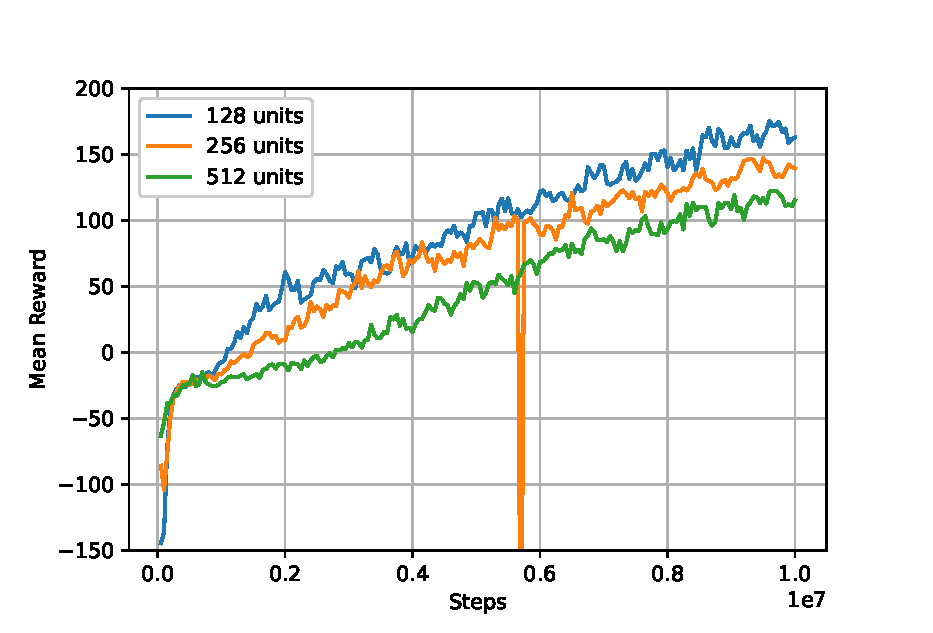
\includegraphics[width=0.95\linewidth]{shoot_moving_target_3_layers.eps}
        \caption{Training results for shooting a moving target with a network with 3 hidden layers}
        \label{train_results_shoot_3_layers}
    \end{center}
\end{figure}

Training the agent with a network with 5 layers obtains the results that can be seen in Figure \ref{train_results_shoot_5_layers} and Table \ref{shoot_moving_targets_table:1}. The situation is similar to the previous ones, meaning that the configuration with 128 units still performs the best. It is better by $1.76\%$ than the one with 256 units and better by $29.38\%$ than the one with 512 units per layer.

\begin{figure}
    \begin{center}
        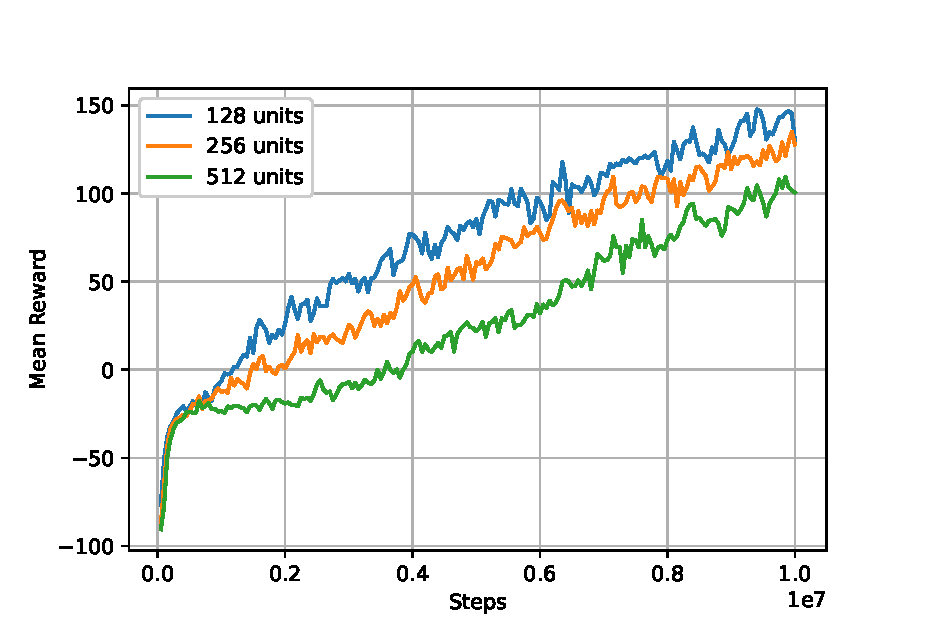
\includegraphics[width=0.95\linewidth]{shoot_moving_target_5_layers.eps}
        \caption{Training results for shooting a moving target with a network with 5 hidden layers}
        \label{train_results_shoot_5_layers}
    \end{center}
\end{figure}

Results for training the agent with 7 network layers can be seen in Figure \ref{train_results_shoot_7_layers} and Table \ref{shoot_moving_targets_table:1}. Again, as in the previous cases, the configuration with the smallest number of units per layer performs better than the other ones during training. The configuration with 128 units performs better by $10.76\%$ than the one with 256 units, and better by $29.09\%$ than the one with 512 units per layer.

\begin{figure}
    \begin{center}
        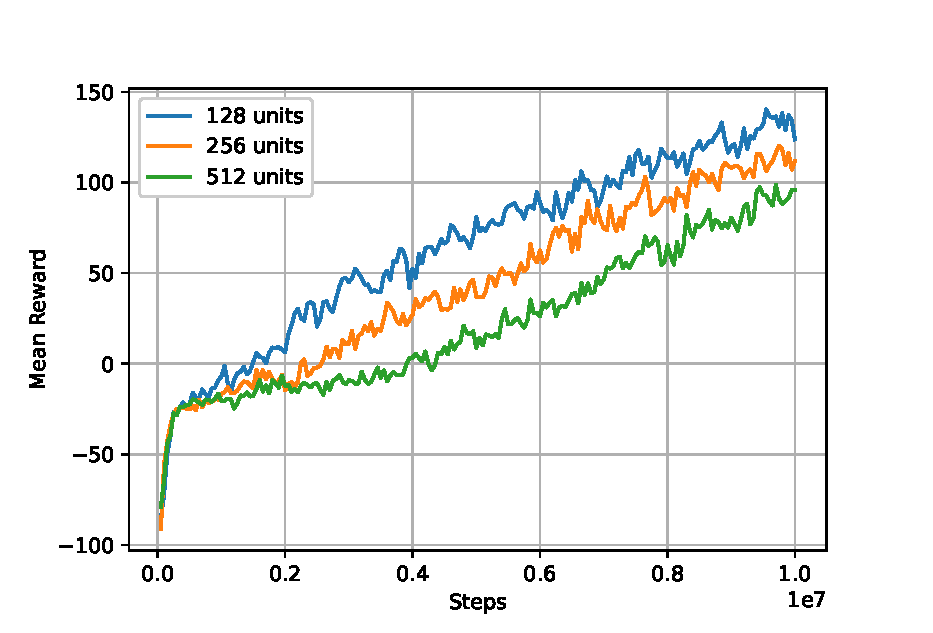
\includegraphics[width=0.95\linewidth]{shoot_moving_target_7_layers.eps}
        \caption{Training results for shooting a moving target with a network with 7 hidden layers}
        \label{train_results_shoot_7_layers}
    \end{center}
\end{figure}

The final results for all configurations can be seen in Figure \ref{train_results_shoot_bar_chart} and Table \ref{shoot_moving_targets_table:1}. From here we can deduce that using a smaller network with fewer units per layer gives the best results during training. Increasing the number of layers decreased the performance of the agent in every single case by up to $\sim40\%$. Thus, it can be clearly infered that using a network architecture with 1 layer and 128 units per layer should give the best performance of the agent, and also use the least amount of computing resources.

\begin{table}
    \centering
    \begin{tabular}{|| m{15em} | m{15em} ||}
    \hline \hline
    \strong{Network Configuration} & \strong{Final Mean Reward} \\ \hline \hline
    1 layer, 128 units & 183.278 \\ \hline
    1 layer, 256 units & 138.719 \\ \hline
    1 layer, 512 units & 166.612 \\ \hline
    3 layers, 128 units & 162.629 \\ \hline
    3 layers, 256 units & 139.293 \\ \hline
    3 layers, 512 units & 115.129 \\ \hline
    5 layers, 128 units & 130.032 \\ \hline
    5 layers, 256 units & 127.781 \\ \hline
    5 layers, 512 units & 100.497 \\ \hline
    7 layers, 128 units & 123.777 \\ \hline
    7 layers, 256 units & 111.752 \\ \hline
    7 layers, 512 units & 95.882 \\ \hline \hline
    \end{tabular}
    \caption{Final training results for shooting a moving target}
    \label{shoot_moving_targets_table:1}
\end{table}

\begin{figure}
    \begin{center}
        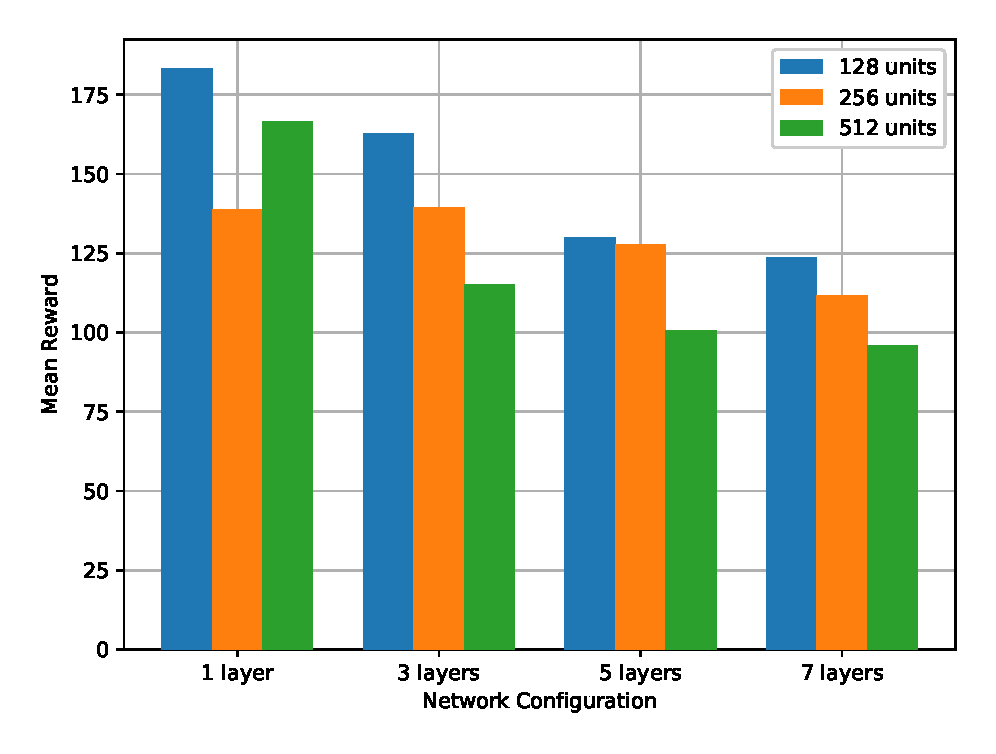
\includegraphics[width=\linewidth]{shoot_moving_target_bar_chart.eps}
        \caption{Training results for all network configurations for shooting a moving target}
        \label{train_results_shoot_bar_chart}
    \end{center}
\end{figure}

\paragraph{}
In the second part of the trainings, the agent is trained using a configuration of 128 units per network layer, since this yielded the best results in the previous phase, and different observations regarding the bullet. The first observation combination uses all three bullet observations: if the bullet is fired, its trajectory vector and its speed; the second observation combination contains only two bullet observations: the bullet's speed and if the bullet is fired; and the final combination contains only the observation that tells if the bullet was fired. This comparison is made to see if adding more observations would increase the agent's performance, or decrease it, similar to what happened when adding the target's movement direction to the observations in Section \ref{moving_target:training}.

Results for training the agent with a single network layer can be seen in Figure \ref{train_results_shoot_obs_comparasion_1_layers} and Table \ref{shoot_moving_targets_table:2}. All 3 observation combinations yield very similar results, with the variant that observes only if the bullet is fired being slightly better then the other two. It is better by $16.91\%$ than the observation combination with both bullet trajectory and speed, and better by $10.12\%$ than the combination with the bullet's speed.

\begin{figure}
    \begin{center}
        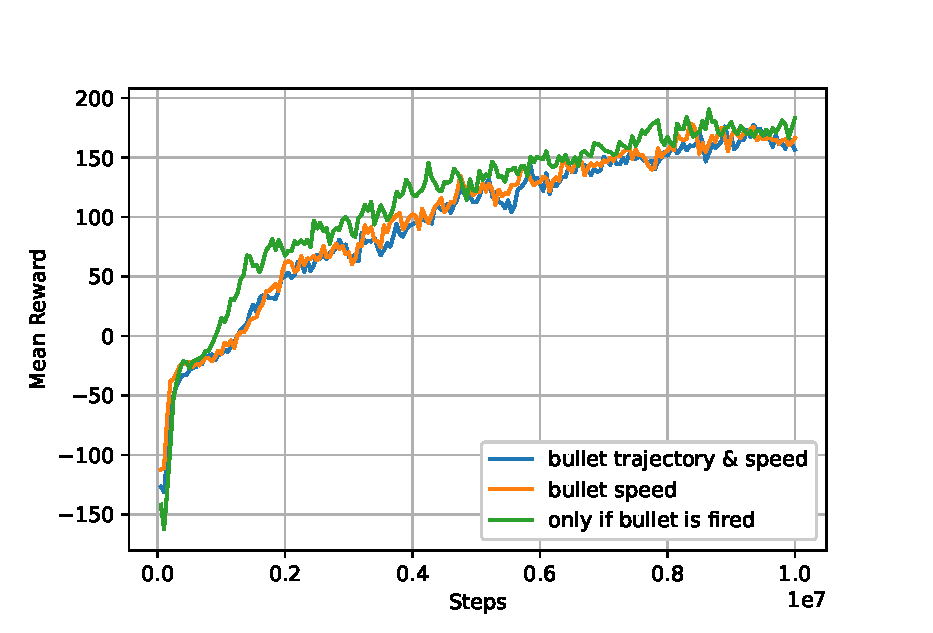
\includegraphics[width=0.95\linewidth]{shoot_moving_target_128_1_layers.eps}
        \caption{Training results for shooting a moving target with a network with 1 hidden layer, 128 units, and different observations}
        \label{train_results_shoot_obs_comparasion_1_layers}
    \end{center}
\end{figure}

The results for training the agent with 3 network layers are in Figure \ref{train_results_shoot_obs_comparasion_3_layers} and Table \ref{shoot_moving_targets_table:2}. Here, it is similar to the previous situation, with all 3 combinations achieving similar training results. Here, the combination with the bullet's speed is the best one, being better by $0.41\%$ than the combination that observes only if the bullet is fired, which means these two combinations obtain virtually identical results, and better by $7.3\%$ than the combination with both bullet trajectory and speed.

\begin{figure}
    \begin{center}
        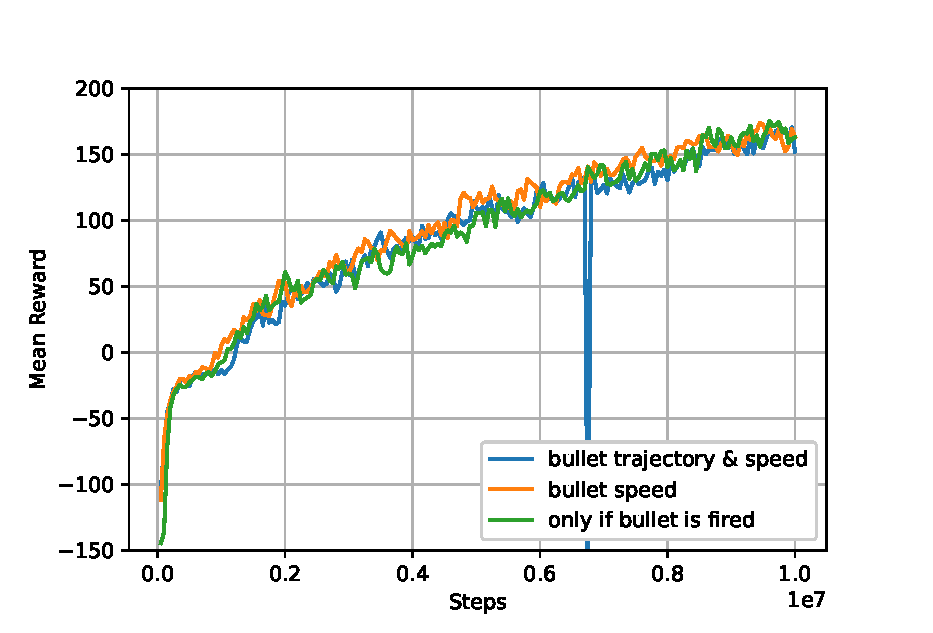
\includegraphics[width=0.95\linewidth]{shoot_moving_target_128_3_layers.eps}
        \caption{Training results for shooting a moving target with a network with 3 hidden layers, 128 units, and different observations}
        \label{train_results_shoot_obs_comparasion_3_layers}
    \end{center}
\end{figure}

Training the agent with a network with 5 layers obtains the results that can be seen in Figure \ref{train_results_shoot_obs_comparasion_5_layers} and Table \ref{shoot_moving_targets_table:2}. Again, training results are very similar for all 3 combinations. Here, the best one is the combination with both bullet trajectory and speed being better by $11.69\%$ than the combination with the bullet's speed, and better by $18.01\%$ the the one that only observes if the bullet was fired.

\begin{figure}
    \begin{center}
        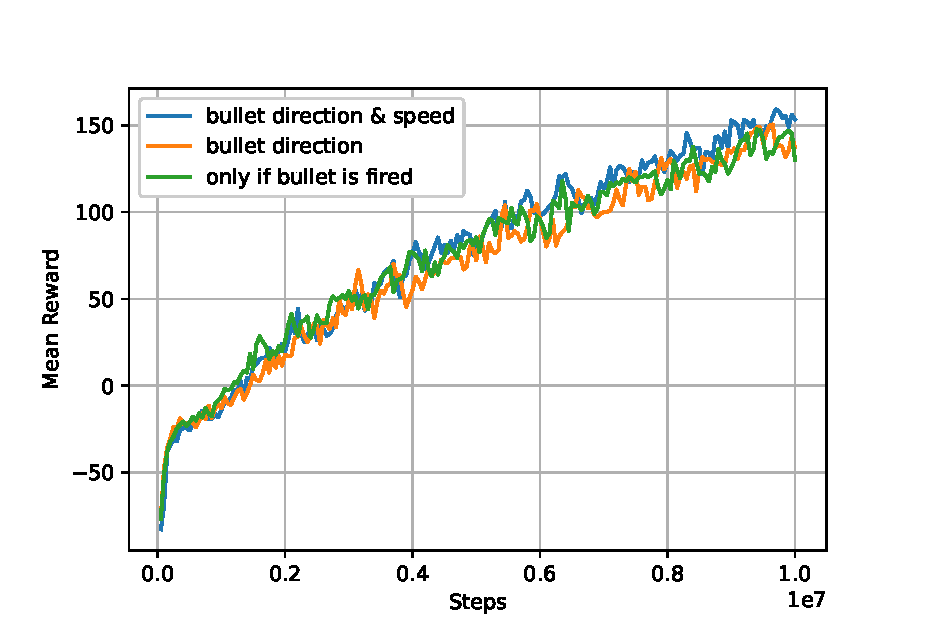
\includegraphics[width=0.95\linewidth]{shoot_moving_target_128_5_layers.eps}
        \caption{Training results for shooting a moving target with a network with 5 hidden layers, 128 units, and different observations}
        \label{train_results_shoot_obs_comparasion_5_layers}
    \end{center}
\end{figure}

Results for training the agent with 7 network layers can be seen in Figure \ref{train_results_shoot_obs_comparasion_7_layers} and Table \ref{shoot_moving_targets_table:2}. All 3 combinations perform virtually identically having a maximum difference in agent performance of $\sim3\%$.

\begin{figure}
    \begin{center}
        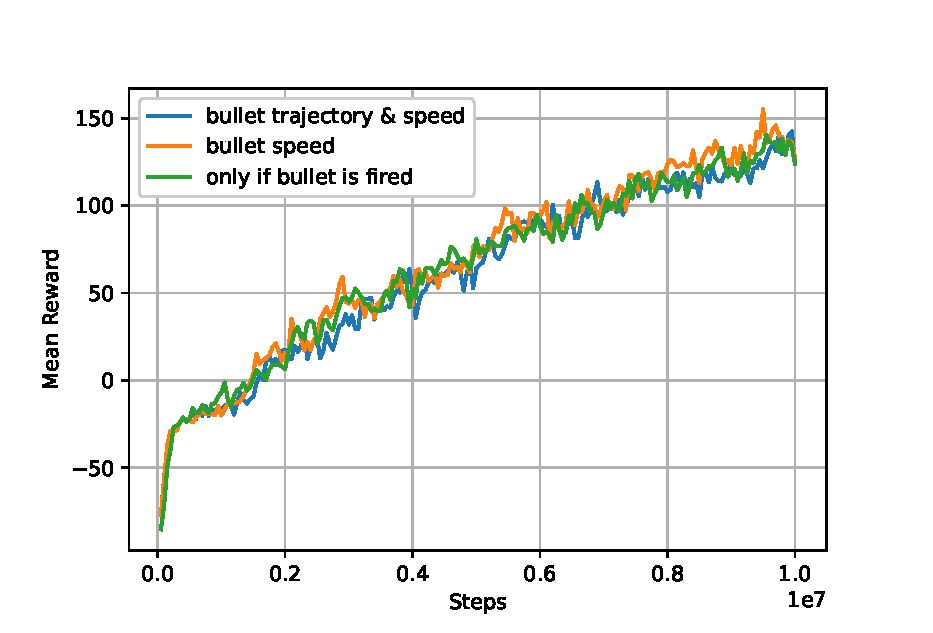
\includegraphics[width=0.95\linewidth]{shoot_moving_target_128_7_layers.eps}
        \caption{Training results for shooting a moving target with a network with 7 hidden layers, 128 units, and different observations}
        \label{train_results_shoot_obs_comparasion_7_layers}
    \end{center}
\end{figure}


The final results for all configurations can be seen in Figure \ref{train_results_shoot_obs_comparasion_bar_chart} and Table \ref{shoot_moving_targets_table:2}. As with the first training stage, increasing the number of layers leads to a poorer performing agent. Also, there were no huge differences when introducing the new bullet observations, with the new observation combinations performing the same or slightly worse then when observing only if the bullet was fired. The only exception is when using a network with 5 layers, where adding the bullet's trajectory and speed to the observations obtains a performance that is $18.01\%$ better than if not including them. However, the best performing configuration still remains the one with 1 layer, and where the only observation about the bullet is if it was fired.

\begin{table}
    \centering
    \begin{tabular}{|| m{12em} | m{13em} | m{10em} ||}
    \hline \hline
    \strong{Network Configuration} & \strong{Bullet Observations} & \strong{Final Mean Reward} \\ \hline \hline
    1 layer, 128 units & Bullet's trajectory and speed & 156.766 \\ \hline
    1 layer, 128 units & Bullet's speed & 166.427 \\ \hline
    1 layer, 128 units & Only if bullet was fired & 183.278 \\ \hline
    3 layers, 128 units & Bullet's trajectory and speed & 152.188 \\ \hline
    3 layers, 128 units & Bullet's speed & 163.311 \\ \hline
    3 layers, 128 units & Only if bullet was fired & 162.629 \\ \hline
    5 layers, 128 units & Bullet's trajectory and speed & 153.46 \\ \hline
    5 layers, 128 units & Bullet's speed & 137.391 \\ \hline
    5 layers, 128 units & Only if bullet was fired & 130.032 \\ \hline
    7 layers, 128 units & Bullet's trajectory and speed & 125.061 \\ \hline
    7 layers, 128 units & Bullet's speed & 127.677 \\ \hline
    7 layers, 128 units & Only if bullet was fired & 123.777 \\ \hline \hline
    \end{tabular}
    \caption{Final training results for shooting a moving target with different bullet observations}
    \label{shoot_moving_targets_table:2}
\end{table}

\begin{figure}
    \begin{center}
        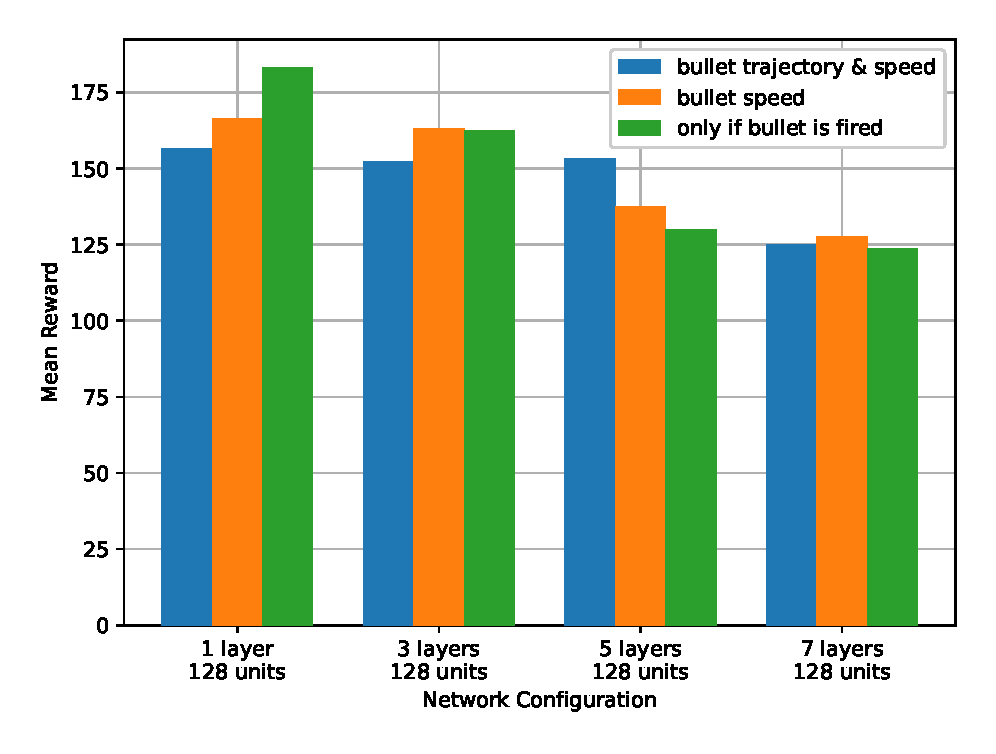
\includegraphics[width=\linewidth]{shoot_moving_target_obs_comparasion_bar_chart.eps}
        \caption{Training results for network configurations with 128 units per layer and different bullet observations, for reaching a moving target}
        \label{train_results_shoot_obs_comparasion_bar_chart}
    \end{center}
\end{figure} 


\paragraph{}
In conclusion, when comparing the two approaches of adding or not multiple bullet observations, it seems that the best results are obtained when observing only if the bullet was fired. When the number of layers increseas, it looks like there is a tendency to obtain better results when adding more bullet observations. However, these results are still worse than when using a network architecture with 1 hidden layer, 128 units per layer, and the only bullet observation is if it was fired.


\subsubsection{Tactical approach} \label{subsubsection:shoot_tactical}

This approach tries to mimic a more realistic fighting scenario, where the target would shoot back at the agent. Thus, through the newly added punishments, described in Formulae \ref{punishment:shoot_1} and \ref{punishment:shoot_2}, the agent should learn to keep a certain distance from the target, and also to flank it. Here, the only bullet observation that is made, is if the bullet was fired or not. This decision was made based on the training results obtained when training the agent in a more \emph{naive} way, in the above experiment. Also, introducing more observations would require the agent to train for a larger number of steps to efficiently use them, if possible, and since the number of training steps still remains $10^7$, and new penalties were added, this would lead to a poorer performing agent. 

\paragraph{}
Results for training the agent with a single network layer can be seen in Figure \ref{train_results_shoot_v2_1_layers} and Table \ref{shoot_moving_targets_v2_table:1}. The configurations with 256 and 512 units per layer had similar perofrmances during the training, however the one with 128 units began to fall behind these two at around $6 \cdot 10^6$ steps. The best performing configuration was the one with 256 units.

\begin{figure}
    \begin{center}
        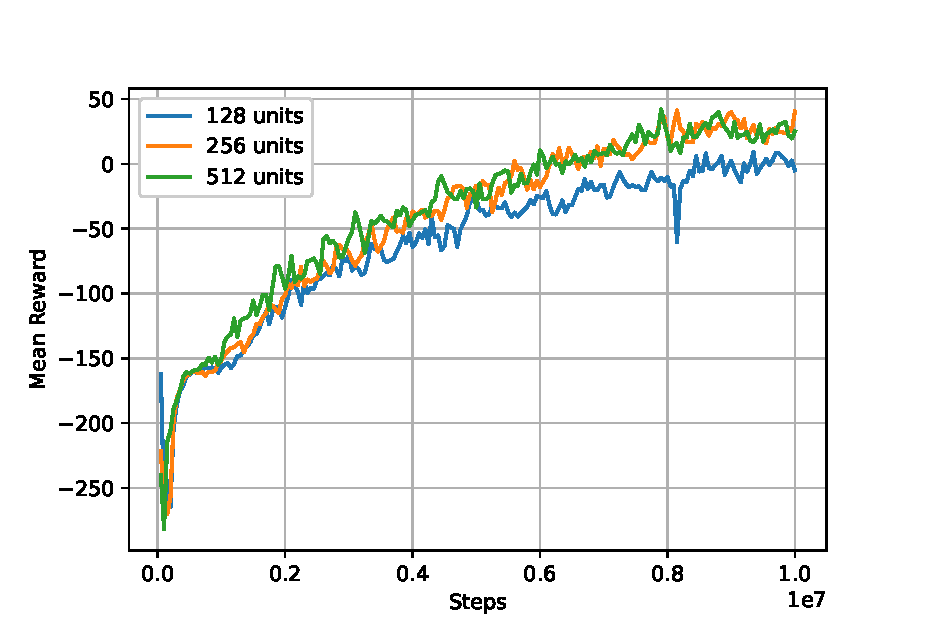
\includegraphics[width=0.95\linewidth]{shoot_moving_target_v2_1_layers.eps}
        \caption{Training results for shooting a moving target with a network with 1 hidden layer}
        \label{train_results_shoot_v2_1_layers}
    \end{center}
\end{figure}

The results for training the agent with 3 network layers are in Figure \ref{train_results_shoot_v2_3_layers} and Table \ref{shoot_moving_targets_v2_table:1}. The configurations with 128 and 256 units per layer performed virtually identically during the training, with the best one being the configuration with 128 units, while the one with 512 units managed to fall behind them from the beginning.

\begin{figure}
    \begin{center}
        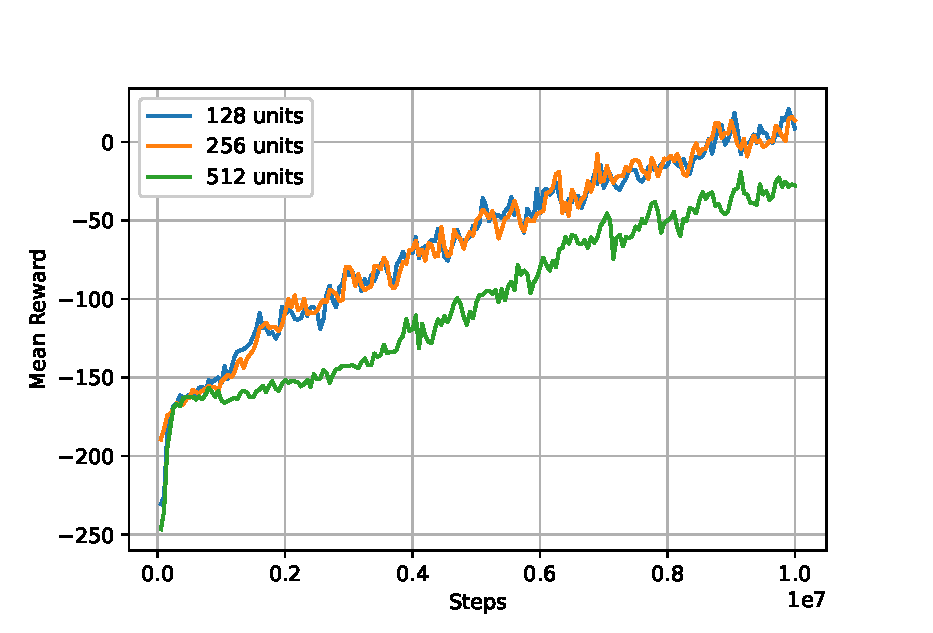
\includegraphics[width=0.95\linewidth]{shoot_moving_target_v2_3_layers.eps}
        \caption{Training results for shooting a moving target with a network with 3 hidden layers}
        \label{train_results_shoot_v2_3_layers}
    \end{center}
\end{figure}

Results for training the agent with 5 network layers can be seen in Figure \ref{train_results_shoot_v2_5_layers} and Table \ref{shoot_moving_targets_v2_table:1}. During the training, the configuration with 128 units per layer performs better than the one with 256 units, while the one with 512 falls behind these two by a large amount.

\begin{figure}
    \begin{center}
        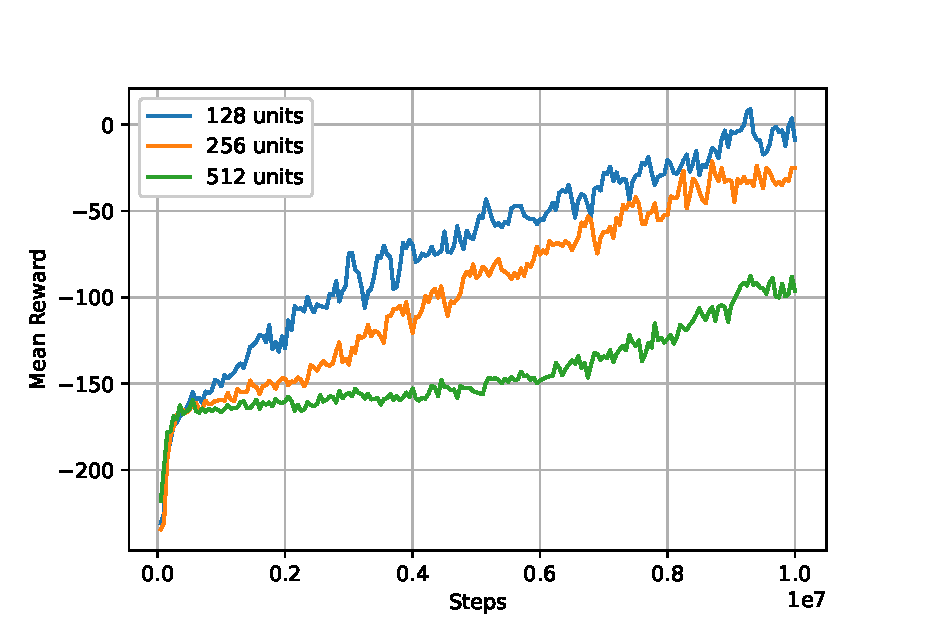
\includegraphics[width=0.95\linewidth]{shoot_moving_target_v2_5_layers.eps}
        \caption{Training results for shooting a moving target with a network with 5 hidden layers}
        \label{train_results_shoot_v2_5_layers}
    \end{center}
\end{figure}

Training the agent with a network with 5 layers obtains the results that can be seen in Figure \ref{train_results_shoot_v2_7_layers} and Table \ref{shoot_moving_targets_v2_table:1}. The results are similar to the ones obtained with an architecture with 5 hidden layers with the configuration with 128 units per layer performing better than the one with 256 units, and the one with 512 units greatly falling behind these two.

\begin{figure}
    \begin{center}
        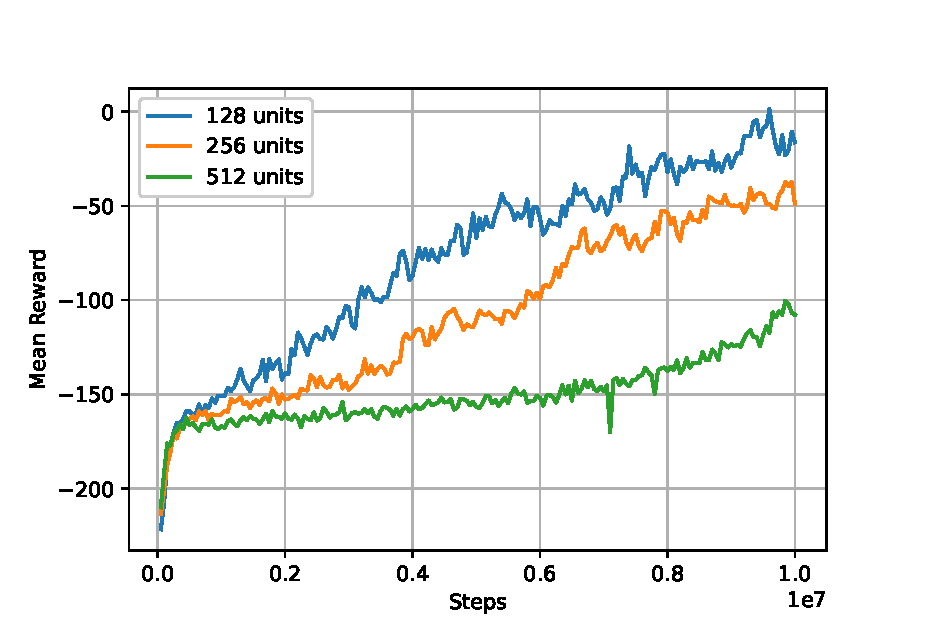
\includegraphics[width=0.95\linewidth]{shoot_moving_target_v2_7_layers.eps}
        \caption{Training results for shooting a moving target with a network with 7 hidden layers}
        \label{train_results_shoot_v2_7_layers}
    \end{center}
\end{figure}


\paragraph{}
In summary, for this type of agent, a smaller network architecture should be used, since it obtains better results, with networks with over 3 hidden layers having a heavily readuced performance. Also, configurations with over 128 units per layer should be used, since the ones with 128 units perform worse in comparison to the others, but only when the number of hidden layers is small.

\begin{table}
    \centering
    \begin{tabular}{|| m{15em} | m{15em} ||}
    \hline \hline
    \strong{Network Configuration} & \strong{Final Mean Reward} \\ \hline \hline
    1 layer, 128 units & -4.727 \\ \hline
    1 layer, 256 units & 40.452 \\ \hline
    1 layer, 512 units & 25.225 \\ \hline
    3 layers, 128 units & 8.479 \\ \hline
    3 layers, 256 units & 13.789 \\ \hline
    3 layers, 512 units & -27.845 \\ \hline
    5 layers, 128 units & -8.788 \\ \hline
    5 layers, 256 units & -25.076 \\ \hline
    5 layers, 512 units & -96.232 \\ \hline
    7 layers, 128 units & -16.319 \\ \hline
    7 layers, 256 units & -48.976 \\ \hline
    7 layers, 512 units & -107.791 \\ \hline \hline
    \end{tabular}
    \caption{Final training results for shooting a moving target}
    \label{shoot_moving_targets_v2_table:1}
\end{table}

\begin{figure}
    \begin{center}
        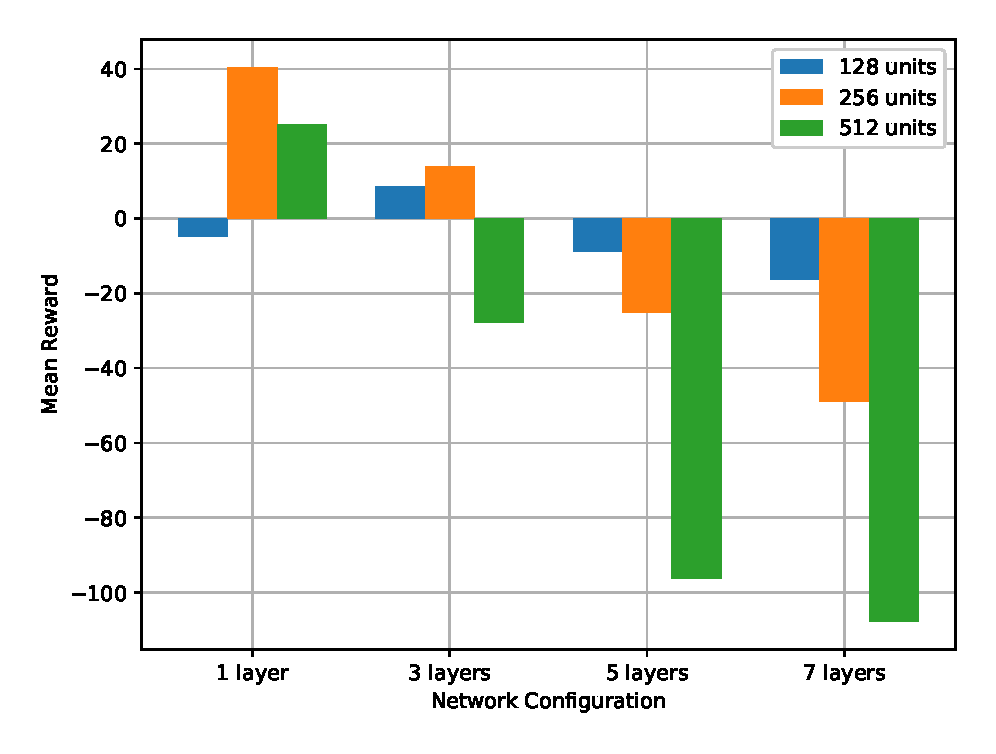
\includegraphics[width=\linewidth]{shoot_moving_target_v2_bar_chart.eps}
        \caption{Training results for all network configurations for shooting a moving target}
        \label{train_results_shoot_v2_bar_chart}
    \end{center}
\end{figure}